\documentclass[../root.tex]{subfiles}

\begin{document}

\section{Introduction}
\label{sec:introduction}

Industrial \emph{robots} are programmed to perform highly specialized and
repetitive actions in controlled environments. Therefore, their
autonomy is quite limited and they are restricted to a small set of
problems. We would like that robots that are
not in such controlled scenarios are able solve a larger variety of
problems, and even to react in the presence
of adverse events.
In other words, we
would like robots to reason about their environment and about the
potential effects that their actions may exert on it.
Such capabilities would allow for great flexibility in the following
ways: (1) tasks can be switched without reprogramming; (2) multiple
solutions to the same problem can be found and assessed in terms
of risk and potential gains in execution speed or other criteria; and (3)
contingency mechanisms can be applied, should adverse events hinder
the execution of the task.

We can think of several applications that are potential targets
of these desirable qualities. One possibility is to use robots to assist old and
impaired people for household chores
or treatment~\cite{canal2018adapting,andriella2018deciding}. Another
application is to allow robots to perform maintainance in difficult-to-access
environments, such as subaquatic facilities~\cite{palomeras2016toward,ong2010planning}.

In this document we are concerned with \emph{automatically disassembly}
of electronic devices with a robotic arm. Namely, we want to enable the
robot to retrieve the most valuable and/or dangerous components.
The recycling application is very exciting both from a scientific
and environmental one, as we will see below. Our intention is
to provide strategies for performing intelligent action selection.
That is, given a disassembly scenario, the robot should be able
to perform the most suitable action taking into consideration
risk and speed criteria. We tackle this objective using tools
from the area of \emph{Automatic Planning and Scheduling}.

\section{Motivation}

The research presented in this document has been conducted aiming at
developing techniques that can be effectively employed to \emph{recycle}
contraptions such as hard drives, hair trimmers, remote controls or
electronic toys. Fig.~\ref{fig:examples-of-devices} shows some
examples of the devices that we have in mind.

\begin{figure}[tbhp]
	\centering
	\begin{subfigure}[b]{0.31\columnwidth}
		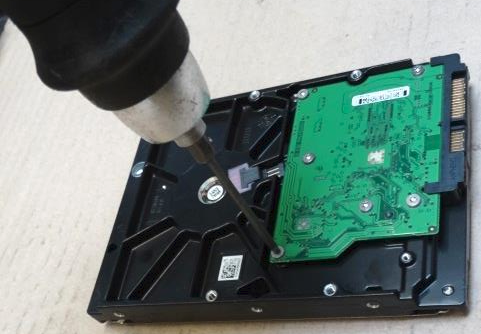
\includegraphics[width=\textwidth]{hddbottom}
		\caption{}
	\end{subfigure}
	~
	\begin{subfigure}[b]{0.31\columnwidth}
		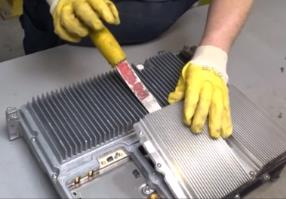
\includegraphics[width=\textwidth]{gsmamp}
		\caption{}
	\end{subfigure}
	~
	\begin{subfigure}[b]{0.31\columnwidth}
		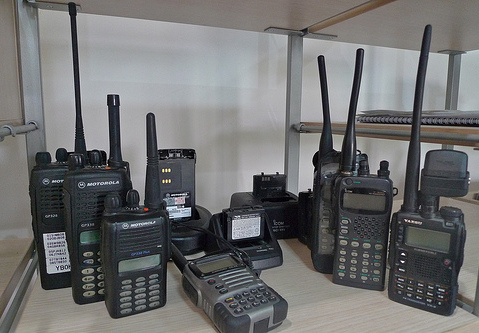
\includegraphics[width=\textwidth]{handies}
		\caption{}
	\end{subfigure}
	\caption{
		(a) Bottom view of a hard drive being disassembled.
		(b) GSM amplifier being disassembled.
		(c) Several handie-talkie models being displayed.
	}
	\label{fig:examples-of-devices}
\end{figure}

In our view, this application poses very attractive challenges
from the scientific point of view. In real-life, deterministic environments
(i.e. fully observable state variables and non-random action outcomes)
are more an exception than a rule, and this becomes evident in disassembly
scenarios. On the one hand, the whole structure of the device cannot be
perceived at once because of occlusions and perception noise, as
Fig.~\ref{fig:examples-of-devices} illustrates. Therefore, progression
in the disassembly task is required to discover hidden components and
geometrical relations. On the other hand, actions might not produce
always the same outcome, due to positioning errors, noise in the movement
of the robots and exogenous factors. For instance, levering the PCB
of a hard drive in order to extract it from the bay might not success
entirely, leaving the PCB hovering over one of the edges of the casing.
In such case, one may need to consider an additional action like levering
from a different point or holding the case upside down to let the loosen
component fall.

\begin{figure}[tbhp]
	\centering
	\begin{subfigure}[b]{0.45\columnwidth}
		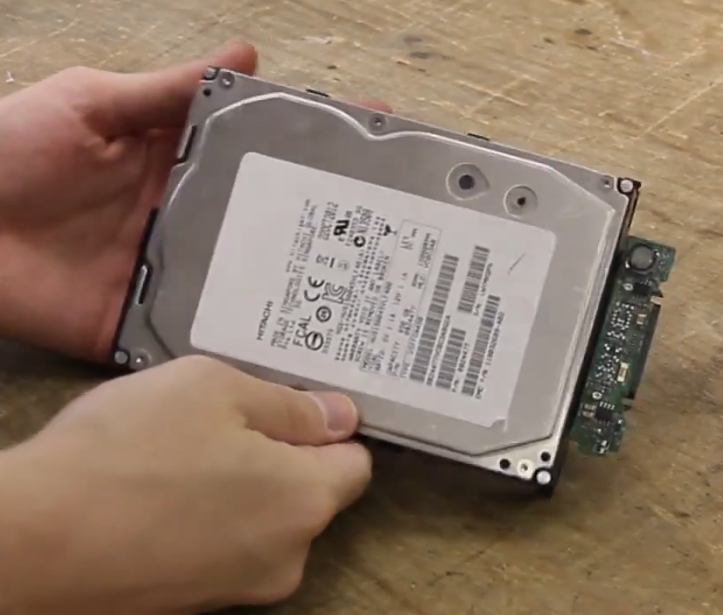
\includegraphics[width=\textwidth]{hddtopcover}
		\caption{}
	\end{subfigure}
	~
	\begin{subfigure}[b]{0.45\columnwidth}
		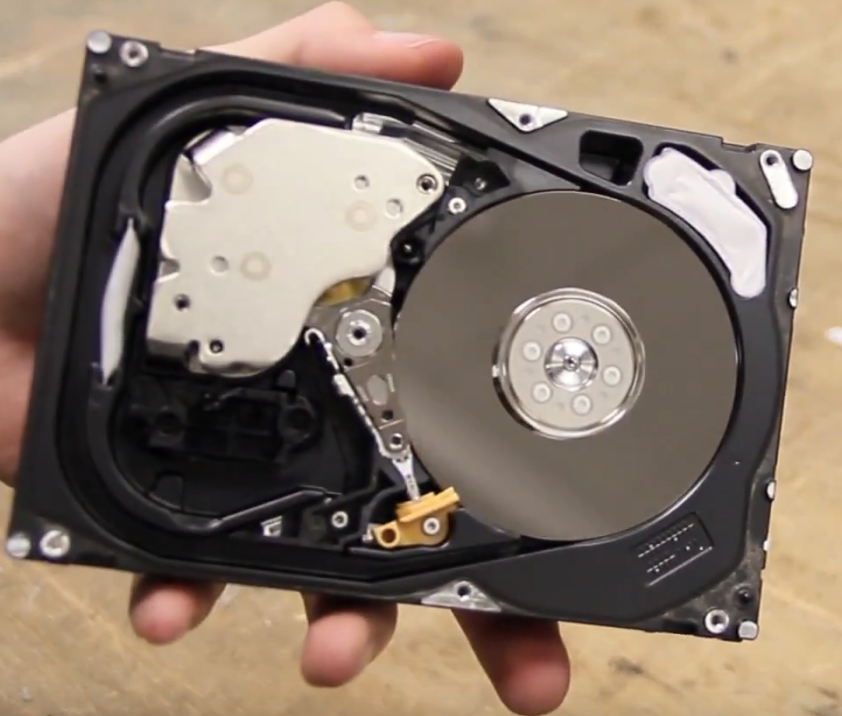
\includegraphics[width=\textwidth]{hddtopwocover}
		\caption{}
	\end{subfigure}
	\caption{
		(a) Top view of a hard drive with the lid.
		(b) View from the same perspective without the lid. The
		previously occluded inner components are now visible.
	}
	\label{fig:example-of-occlusion}
\end{figure}

We cannot forget either the social and environmental impact of the
proposed application. The current recycling industry is dominated
by the \emph{crush and separate} paradigm. Trash is crushed into
very small bits that are then filtered and classified using
physical properties such as density or inductance. However,
the uniformity of the separated debris cannot be guaranteed.
Even more importantly, devices often contain components or
substances that are hazardous for the environment. In such cases,
it is required that a human manually removes the source of danger.
This has associated health risks for the operator. Moreover,
it is inefficient and costly, so a great amount of trash is
simply incinerated, posing a serious thread for the ecosystems.
Another drawback of this method is that precious or reusable
components (e.g. PCBs, capacitors, magnets...) are destroyed,
when they can be used right away or after some refurnishing
in the manufacturing of new products.

In light of these arguments, a robotic recycling system is
appealing from the sustainability perspective as well.
To avoid the drawbacks of the \emph{crush and separate} method,
we would like the following features for the robot:
(1) it should
ideally adapt to different electromechanical contraptions
(including different brands/models of the same device);
(2) it should correctly identify the tasks that it
has to complete to perform a successful disassembly; and (3)
it should be able to work even with damaged devices.

\section{Involvement in H2020 Imagine}

This research has been conducted as part of the European H2020 project
\emph{Imagine: Robots Understanding Their Actions by Imagining Their Effects},
or just \emph{Imagine}\footnote{\url{https://imagine-h2020.eu/}}. The scientific
objective of \emph{Imagine} is to make robots aware of their environment
and, in general, to achieve the autonomy objectives discussed
previously in
Section~\ref{sec:introduction}. The project focuses on the recycling
application introduced in the former section.

There are seven European research centers participating in \emph{Imagine},
each working on a different subsystem. One of these subsystems is a
planning and decision unit, which is developed by the IRI-CSIC 
(\emph{Institut de Rob\`otica i Inform\`atica Industrial}%
\footnote{\url{http://www.iri.upc.edu/}}-%
\emph{Consejo Superior de Investigaciones Cient\'ificas}%
\footnote{\url{http://www.csic.es/}}) partner. This thesis is hosted
in this institution and is closely
related to the development of the \emph{Imagine}'s decision unit.
This subsystem is a fundamental part of the overall system, since it
evaluates the scene and selects the action that is more suitable for
the perceived state. This means that it has to make sure that the action
is beneficial in the long term and that the risk of falling into a
dead end is controlled.

The project also features PHYS and ASC as novel ideas for the considered application.
The first is a very realistic and
powerful physics simulator that can give a very precise idea of the state that results
from executing an action, but makes intensive use of
computational resources. The second is an Association Engine that identifies the
points of interest
of the scene, and also learns a high level physics model (``folks physics'')
that is much quicker to invoke than PHYS, but also less accurate.
They are very useful and have great potential, because the planner can interact
with them and ``imagine'' plans before any action.
Another key aspect of the project is the concept
of ADES, or \emph{Action Description}, for storing the symbolic description
of the actions and the DMPs (\emph{Dynamic Movement Primitive}) associated to
each one. Other aspects of the project include the perception of the scene
and the design and construction of a multifunctional gripper.

\begin{wrapfigure}{L}{0.5\columnwidth}
	\centering
	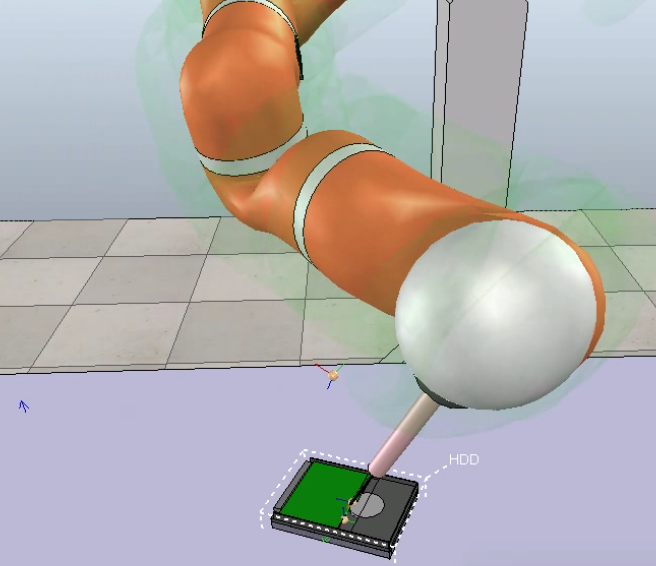
\includegraphics[width=\linewidth]{vrepimage}
	\caption{Execution of a levering action in the V-REP simulator.}
	\label{fig:vrepimage}
\end{wrapfigure}

As of today, we have been participating actively on \emph{Imagine} for more
than a year.
In April of 2018 the project was evaluated by a Project Officer and three experts in
different areas of robotics. It received very positive critics. Part of the
presentation for the evaluation meeting consisted in a demonstration that
displayed basic prototypes of the different subsystems interacting with each
other, and was
able to solve very simple disassembly simulated scenarios
involving a
hard drive (see Fig.~\ref{fig:vrepimage}).
This demonstration already featured a planner prototype in the loop.
Our objectives for this year is to extend this planner with new
capabilities, including the ones presented here, but also with
a rich and beneficial interaction with PHYS and ASC.

\section{Related concepts}

We see in the area of \emph{Automatic Planning and Scheduling}
tools that potentially bring us toward the
desirable qualities exposed above.
Planning is a branch inside Artificial
Intelligence that aims at solving problems that are defined
\emph{declaratively}, with as little control (procedural) knowledge
as possible.
That is, a
planning algorithm
operates with a model that encodes the dynamics of the domain and, for
each problem, outputs
an action sequence
or a policy that solves it, has a high success probability or has a high
expected reward.

%Since Automatic Planning deals with optimizing an agent's
%behavior to operate in a certain environment, it is possible to see some
%similarities between planning and Reinforcement Learning. The main difference
%is that, in their most basic form, a Reinforcement Learning agent is
%model-free and dependent on its learning capabilities to decide the
%suitable action for a certain state, while a planner takes advantage of a
%model of the domain and employs informed search or other heuristic methods to
%find a plan (although definitively there
%exist works that allow partial domains and that incorporate learning
%capabilities to complete these them~\cite{martinez2017relational,martinez2015vmin}).

It is worth saying that planning is not a discipline that is particular to
robotics and, therefore, there exist multiple benchmarks and work in the
field that is general enough to be of use in many areas. One of the
most successful conferences that spreads knowledge in the field of planning is
ICAPS (International Conference in Automatic Planning and Scheduling)
\footnote{\url{http://www.icaps-conference.org/}}. The conference is
held every year and hosts a competition that seeks to push the boundaries
of the state of the art planning systems.

\section{Approach}

We will resort to the MDP (\emph{Markov Decision Process})
formalism to express our problem, capturing the uncertainty over
the state transitions.
One of the main limitations of MDPs for
real-life problems is that they assume full observability of the state variables.
In practice, this is not true for our application. However, dropping this
assumption results in POMDPs
(\emph{Partially Observable MDPs}), whose resolution is computationally costly
and scales badly with the size of the state space. Moreover, POMDPs are
still difficult to apply when the agent does not know all
the variables of the state (which may happen when the it is not aware of all
the relevant objects of the scene).

We update and solve a new MDP each
time the specification of the state changes (i.e. when new objects are discovered
after performing an action). Even though solving MDPs is much less intensive than
solving POMDPs, conventional algorithms such as \emph{Value Iteration} and
\emph{Policy Iteration} still suffer from the curse of dimensionality when there
are many state variables. Then, computing a full policy becomes infeasible.
We explore two complementary strategies for dealing with this: (1)
determinization algorithms together with classical planners; and (2)
decompositon of the main goal into sub-goals, taking advantage of the
topological precedences imposed by some circumstances (e.g. partial
occlusion).

\section{Scope and goals}

The present work revolves mainly around probabilistic planning, without focusing too much
on topics such as scene perception and low-level robot control.
We present tools for modeling stochastic problems from the recycling
domain, as well as techniques for
dealing efficiently with these problems. Although all the examples and benchmarks
have been conceived for the particular use case of the hard drive,
the techniques described here can be extrapolated to other devices by extending
the state specification with variables particular to these devices.
We focus on the use case of the
hard drive disassembly.

More specifically we:
\begin{itemize}
	\item propose a set of predicates to represent the different components of
	the device and their relation to other components. These are used to represent
	the world state.
	\item propose a PPDDL (\emph{Probabilistic Planning Domain Definition Language})
	model for the recycling domain. This model contains the schemata of the actions
	that can be applied in the domain, as well as the specification of the
	state variables (predicates and functions). PPDDL defines an action-based
	DBN (\emph{Dynamic Bayes Network}) with full observability or, equivalently,
	a MDP.
	\item explore and test several determinization techniques to achieve fast
	approximate on-line solutions to MDPs. The rationale is to avoid costly policy
	recalculations each time the state specification changes when new objects
	are discovered (e.g. after removing the lid of a hard drive). The considered
	determinization algorithms are: (1) All-Outcome and Single-Outcome;
	(2) Alpha-Cost Transition Likelihood; (3) Hindsight optimization.
	\item complement the previous technique with hierarchical planning, taking
	advantage of the strong precedences that arise naturally in the
	considered application. This occurs, for instance, when the read
\end{itemize}

We assess the effectiveness of these strategies testing them against
benchmark problems. On the one hand, we have all the problems from past
IPPCs
(\emph{International Probabilistic Planning Competitions}, hosted
each year by the ICAPS). These are useful to evaluate the suitability of
the different
determinization strategies in domains different from ours. On the other hand,
we have hand-crafted a set of benchmark problems that consist of
hard drive variations with different disposition of components. The determinization
algorithms are evaluated on top of these, too. In addition, these will serve
the purpose of assessing the computional gain of the hierarchical planning
method that is specific for the recycling domain.

\section{Related work}

asdfsadf

\IfEq{\jobname}{\detokenize{root}}{}{\printbibliography}

\end{document}